\graphicspath{{img/ch6}}

\section{Potential for Permanent Human Presence}

\subsection{Natural Advantages of Lunar Pits}

\subsubsection{Radiation and Micrometeoroid Shielding}

Lunar pits provide inherent protection against two significant hazards on the Moon: radiation and micrometeoroid impacts. Without a magnetic field or atmosphere, the lunar surface is exposed to intense solar and galactic cosmic radiation (GCRs) and a constant flux of micrometeoroid impacts. Pits mitigate these threats through their overlying material, which acts as a natural shield.

Studies confirm that radiation levels within pits are significantly reduced compared to surface conditions, akin to the levels inside lava tubes, where overburden thicknesses exceeding 10 meters block high-energy particles \cite{thermal-lunar-pits, newer-thermal}. This protection is essential for safeguarding astronauts from GCRs and solar particle events (SPEs), both of which pose serious health risks over extended periods. Similarly, the steep walls and overhanging entrances of pits intercept micrometeoroids, reducing the risk of structural damage to habitats and equipment \cite{bases-feng, Carrer2024}.

\subsubsection{Thermal Stability and Resource Potential}

Lunar pits exhibit stable thermal environments compared to the Moon’s surface, where extreme temperature fluctuations occur. The geometry of pits limits exposure to direct sunlight and reflected infrared radiation, creating conditions favorable for volatile trapping. Permanently shadowed regions within pits may harbor water ice, a critical resource for long-term human missions, as it can be converted into hydrogen and oxygen for life support and propulsion \cite{jsanders-isru}.

The stable environment also enhances the efficiency and longevity of in-situ resource utilization (ISRU) equipment. Systems for oxygen extraction, regolith processing, and volatile harvesting benefit from reduced maintenance and operational constraints, making pits ideal locations for resource storage and processing \cite{thermal-lunar-pits}.

\subsection{Lunar Base Construction}

\subsubsection{Site Selection and Habitat Design}

Lunar pits are optimal sites for future habitats due to their natural shielding, structural stability, and access to subsurface voids. Prominent candidates include the \textbf{Mare Tranquillitatis} and \textbf{Marius Hills} pits, both of which demonstrate stability, accessibility, and scientific significance \cite{new-wagner, Carrer2024}.

Base designs focus on modular pressurized habitats and inflatable structures, leveraging pits’ overhangs for primary shielding. Advanced proposals involve autonomous rovers reinforcing pit walls with regolith layers or anchoring modular units to the walls using drill-based attachments. These methods minimize reliance on Earth-supplied materials, reducing mission costs and enhancing sustainability \cite{bases-feng}.

\begin{figure}[H]
    \centering
    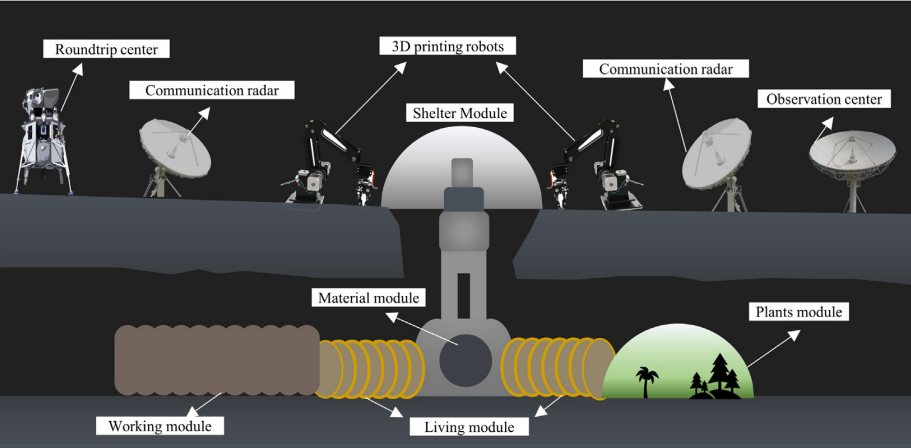
\includegraphics[width=0.75\linewidth]{simple-base-schema.png}
    \caption{Conceptual design of a lunar base within a pit. The natural overhangs provide protection against radiation and micrometeoroid impacts, while modular inflatable habitats offer pressurized living space. The stable environment supports extended operations. Adapted from \cite{bases-feng}.}
    \label{fig:lunar-pit-habitat-concept}
\end{figure}

\subsubsection{Construction and Exploration Strategies}

Before establishing habitats, robotic missions will map and assess pits for stability and resource potential. Tethered climbers, drones, and robotic hoppers, such as the \textbf{Daedalus rover}, will explore pit interiors, identifying structural weaknesses and potential subsurface voids \cite{Carrer2024}. 

Construction will begin with sealing sections of pits to create enclosed, pressurized spaces. Basaltic rock, abundant in pits like Marius Hills, serves as a durable material for habitat foundations. ISRU technologies will play a pivotal role, converting regolith into building materials and ensuring self-sufficiency for long-term habitation \cite{jsanders-isru, new-wagner}.

\subsection{Advanced ISRU Applications}

\subsubsection{Water and Volatile Harvesting}

Regions within pits experiencing permanent shadowing may accumulate water ice and other volatiles. Extraction processes will focus on converting these resources into hydrogen and oxygen via electrolysis, providing essential components for life support systems and propulsion \cite{jsanders-isru}.

\subsubsection{Oxygen and Material Production}

Oxygen extraction from regolith through molten regolith electrolysis or ilmenite reduction will be integral to self-sustaining bases. Pits’ stable conditions reduce mechanical failures, ensuring consistent oxygen production. Additionally, regolith processing enables the creation of construction materials like sintered bricks or 3D-printed modules, further minimizing reliance on Earth-based supplies \cite{bases-feng}.

\subsubsection{Energy and Storage Systems}

Pits provide ideal conditions for energy storage and equipment operation. Their thermal stability reduces energy loss in storage systems and increases the efficiency of ISRU operations. This environment supports continuous resource extraction, processing, and storage, laying the foundation for permanent lunar habitats \cite{thermal-lunar-pits, jsanders-isru}.

\subsection{The Road Ahead: Manned Missions to Lunar Pits}

The potential of lunar pits is already influencing mission planning. Programs like \textbf{NASA’s Artemis} aim to establish sustainable human presence by the 2030s, focusing on polar regions but incorporating learnings from pit exploration. ESA’s \textbf{Daedalus mission} will contribute valuable data on structural stability and internal geometry, shaping future habitat designs. Such missions represent the convergence of robotic and human efforts to unlock the Moon’s potential as a platform for deep space exploration \cite{Carrer2024, jsanders-isru}.